\documentclass[11pt]{article}
\usepackage{graphicx}
\usepackage[utf8]{inputenc}
%\usepackage{polski}
\usepackage{enumerate}
\usepackage{multirow,tabularx}
\usepackage{amssymb}
\usepackage{caption}
\usepackage{multicol}
\usepackage{subfigure}
\usepackage{tikz}
\usepackage{float}
\usepackage[a4paper, left=2cm, right=2cm, top=2cm, bottom=2cm, headsep=1.2cm]{geometry} 
\usepackage[bottom]{footmisc}
\renewcommand{\baselinestretch}{1.1} 
\usepackage{hyperref}
\renewcommand{\familydefault}{\sfdefault} %sans-serif font in entire document expect maths
\usetikzlibrary{er,positioning}

%packages for bash code style
\usepackage{xcolor}
\usepackage{listings}
\lstset{basicstyle=\ttfamily,
  showstringspaces=false,
  commentstyle=\color{blue},
  keywordstyle=\color{red},
  breaklines=true,
  postbreak=\mbox{\textcolor{red}{$\hookrightarrow$}\space},
}

\title{\Huge{Cloud computing} \\ \huge{Simple AWS cluster - configuration, creation, calculations}}
\author{Michal Ranachowski}
\date{2019\\ February}


\begin{document}

\maketitle

\section{Introduction}
The purpose of this paper is to understand basic concept of cluster and go through process of creation cluster Amazon Web Services resources. It was created as part of cloud computing course. This paper is addition to bash script \url{https://github.com/mranachowski/AWS.git} and it describe conceptual layer of creating this type simple cluster. Script is commented inside so combined with this document person with basic knowledge of bash and Linux can easily use it. Calculation costs were covered from AWS Educate grant founds. 

\section{Amazon Web Services}
Amazon Web Services (\textit{AWS}) is on-demand cloud service platform providing computer power, database storage and specialist tools for data processing \footnote{\url{https://aws.amazon.com/what-is-aws}}. It works under AWS Global Infrastructure - data centers spread around the world.\\ \\
\textit{The following section was created based on AWS documentation.\footnote{\url{https://docs.aws.amazon.com}}}

\subsection{AWS first steps}
To begin using service user must create account and perform basic settings in AWS console. This part is not covered in this paper.

\subsection{AWS CLI}
CLI(\textit{Command Line Interface}) is command-line tool for managing Amazon Web Services resources. Combined with bash it allows to create scripts for task automation. On Linux machines it can be easily install through Python Package Installer:
\begin{lstlisting}[language=bash]
$ pip install awscli
\end{lstlisting}
After installation process user must configure AWS CLI, it can be done by execute command and provide necessary credentials and information. It will create default profile.
\begin{lstlisting}[language=bash]
$ aws configure
AWS Access Key ID : 
AWS Secret Access Key : 
Default region name : 
Default output format : 
\end{lstlisting}
The given data is stored in files: \textit{/.aws/credentials} and \textit{/.aws/config}.

\subsection{Used services - EC2 and S3}
\textbf{EC2} - Elastic Compute Cloud provides virtual computing environments, \textit{instances}, which could be treat for imagine purpose as physical machines. It works under Amazon Machine Images (AMI) - "operating system". User can choose from many different hardware configurations: CPU, memory, volume storage. Amazon provides few specialized instances group.\footnote{\url{https://aws.amazon.com/ec2/instance-types/}}\\ \\
\textbf{S3} - Simple Storage Service provide object storage. From the user`s side it is collection of \textit{Buckets} that contain folders. As well as EC2, there are few types of storage classes.\footnote{\url{https://aws.amazon.com/s3/storage-classes/}}

\subsection{Useful concepts}
\subsubsection{Placement group}
There are three type of placement group: \textit{cluster, partition, spread}. \footnote{\url{https://docs.aws.amazon.com/AWSEC2/latest/UserGuide/placement-groups.html}} Cluster ,used in script, logically place group of instances in a single Availability Zone providing high network throughput and low latency communication between instances which is crucial for cluster performance. Placement group creating by AWS CLI:

\begin{lstlisting}[language=bash]
$ aws ec2 create-placement-group --group-name your group name --strategy cluster
\end{lstlisting}

\subsubsection{Security group}
Security group acts like a virtual firewall and controls traffic for instances. When creating instances user must assign security group, instead of default would be apply. By default all inbound traffic is forbidden and all outbound traffic is allowed. By adding rules this settings can be modified. There are rules for communication inside and between security groups and rules for traffic from the Internet (ips, protocols and ports). 

\begin{lstlisting}[language=bash]
$ aws ec2 create-security-group [options]
$ aws ec2 authorize-security-group-ingress [options]
\end{lstlisting}

\subsubsection{IAM}
IAM - \textit{Identity \& Access Management} is service that helps securely control to AWS resources. \textit{\url{https://docs.aws.amazon.com/IAM/latest/UserGuide/introduction.html}}\\
IAM users ale created within one account, and root user should no be use for everyday task, olny for administrative ones. IAM policies are collection of rules and permission. IAM role gives AWS service (for example EC2) permission to act like a user so we can now assign policies to this service. For example necessary when EC2 want to has access to S3 resources.

\subsubsection{Instance skeleton}
Instance skeleton are templates in java script format \textit{.json} which holds many settings for launching instance. Default skeleton is generating by;

\begin{lstlisting}[language=bash]
$ aws ec2 run-instances --generate-cli-skeleton
\end{lstlisting}

\section{Parallel computing}
Parallel computing is a type of computation in which many calculations or the execution of process are carried out simultaneously. \footnote{\url{https://en.wikipedia.org/wiki/Parallel_computing}}. Main idea is to split larger problems (size and/or time consuming) into smaller ones. Parallelism is basis of high-performance computing. There are many type of paralleling and it is large field of nowadays IT technology (hardware and software). In this paper only high-level use of MPI was covered.

\subsection{MPI}
For performing parallel computing on created AWS CLuster MPI was used. MPI stands for \textit{Massage Passing Interface} ad it is communication protocol widely used which became standard for high-performance computing\footnote{\url{https://en.wikipedia.org/wiki/Message_Passing_Interface}}. Originally developed for C, C++ and FORTRAN, but today they are available implementation for most popular programming language. MPICH2 implementation was used in this project. Under Ubuntu installation process:
\begin{lstlisting}[language=bash]
sudo apt-get install mpich
\end{lstlisting}
Main parts of this packages are: \textit{mpicc} - C MPI compiler and \textit{mpiexec} - which allows executing previously compiled files. Below is an example usage of \textit{MPI Hello world} (also given).

\begin{lstlisting}[language=bash]
mpiexec -np NUMBER_OF_PROCESSES -f HOST_FILE ./hello_world\textit{(allready compiled)}
\end{lstlisting}

\begin{lstlisting}[language=c]
#include <stdio.h>
#include <mpi.h>

int main(int argc, char** argv) {
    int myrank, nprocs;

    MPI_Init(&argc, &argv);
    MPI_Comm_size(MPI_COMM_WORLD, &nprocs);
    MPI_Comm_rank(MPI_COMM_WORLD, &myrank);

    printf("Hello from processor %d of %d\n", myrank, nprocs);

    MPI_Finalize();
    return 0;
}
\end{lstlisting}

\section{Using a cluster script}
\begin{figure}[H]
    \centering
    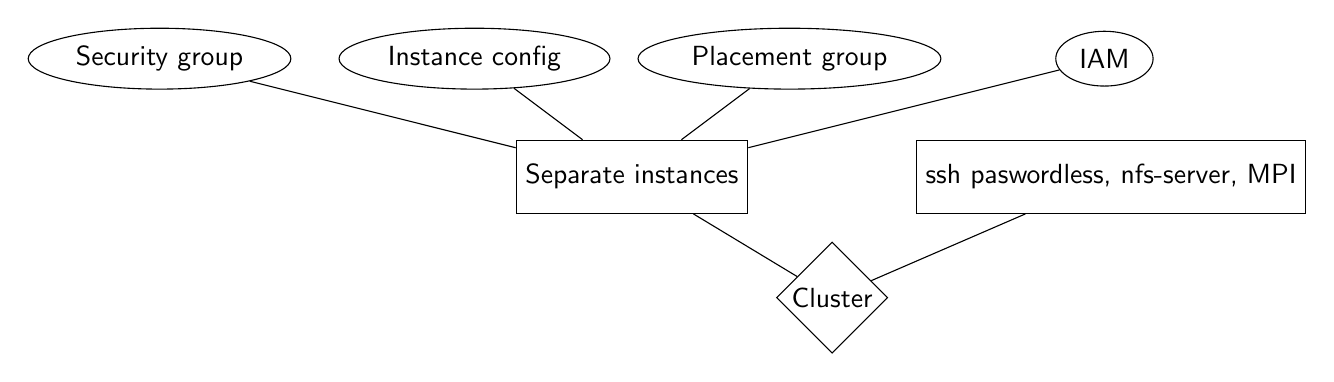
\begin{tikzpicture}[auto,node distance=1cm]
    \node[entity] (node1) {Separate instances}
    [grow=up,sibling distance=4cm]
    child {node[attribute] {IAM}}
    child {node[attribute] {Placement group}}
    child {node[attribute] {Instance config}}
    child {node[attribute] {Security group}};
  \node[relationship] (rel1) [below right = of node1] {Cluster};
  \node[entity] (node2) [above right = of rel1]	{ssh paswordless, nfs-server, MPI};
  \path (rel1) edge node {} (node1) 
        edge	 node {}	(node2);
\end{tikzpicture}
\caption{Schematic diagram of cluster created in this project}
\end{figure}

%\subsection{Files and folder structure}

\subsection{SSH passwordless}
SSH within cluster (eg. master to node) must be setup as passwordless to achive properly working cluster. Standar way to do this is describe in \textbf{\hyperlink{https://help.ubuntu.com/community/MpichCluster}{this tutorial}}. However there is easier way if we created all AWS instances with the same key pair. The solution is \textit{key agent forwarding} and proper ssh configuration on your local machine \footnote{\url{https://www.ssh.com/ssh/agent}}. 

\subsection{Nfs - server and sharing master's folder}
NFS allows to create a folder on the master node and have it synced on all the other nodes \footnote{\url{https://help.ubuntu.com/community/MpichCluster}}. It reduce problem of unnecessary redundancy.  This folder can be used to store programs. 

\subsection{Setup for Linux distribution packages' update and install}
In order to update and install all necessary packages under clean, already installed Linux distribution (in this case Ubuntu 18.04) following command is used:
\begin{lstlisting}[language=bash]
$ sudo DEBIAN_FRONTEND=noninteractive apt-get -y update
$ sudo DEBIAN_FRONTEND=noninteractive apt-get -y install ...
\end{lstlisting}
"DEBIAN\_FRONTED=noninteractive" sets default answer if interactive prompt will appear during package update. "-y" do the same task for ordinary question in terminal.

\section{Parallel computing - structural analysis in Elmer}
To carry out parallel computation which is final task in this project Elmer was choosen, which is open source software multiphisics simulation which uses finite element method to solve phenomena described by partial differential equation. Main advantages which are helpful in this procejt are fact that Elmer is provide as Ubuntu packages repository in MPI compiled version. It is important, because compilation process might take quite a lot time. Installation process:
\begin{lstlisting}[language=bash]
$ sudo apt-add-repository ppa:elmer-csc-ubuntu/elmer-csc-ppa
$ sudo apt-get update
$ sudo apt-get install elmerfem-csc
\end{lstlisting}
Great advantage of Elmer is well documentation\footnote{\url{https://www.csc.fi/web/elmer/documentation}}.
To perform analysis in parallel mode user must execute two commands (all details are describe in Chapter 16 \hyperlink{http://www.nic.funet.fi/pub/sci/physics/elmer/doc/ElmerSolverManual.pdf}{This document}):
\begin{lstlisting}[language=bash]
$ ElmerGrid [option] [option] meshdirectoryname [ mesh partitioning option]
$ mpiexec -np NUMBER_OF_PROCESSES ElmerSolver_mpi
\end{lstlisting}
ElmerSolver\_mpi is recompiled  solver. After excedute this command program will look for ELMERSOLVER\_STARTINFO file which holds links to file containing analysis data.

\end{document}